% !TeX root = ../main.tex
\section{Computational cost}
\label{sec:scalability}

% ===========================================================================
% Evidence: Simulations/Complexity/scaling_20260917/ (benchmark_cost.R, results/timings.csv,
% results/prox_iterations.csv, results/environment.txt, pilot/banded_checks.csv, full_log.txt)
% and notes/complexity_analysis/ (build_tables.py, make_cost_figure.py, summary.json).
% Every number in this section is generated from those files; rerun build_tables.py to
% regenerate the two table bodies and make_cost_figure.py for figures/cost_scaling.pdf.
% ===========================================================================

Section~\ref{sec:simulations} compared estimation accuracy at a single sample size. This section turns to the cost of one complete Gibbs sweep and how it grows with $n$, comparing the individual sampler with the Laplace and horseshoe samplers of \citet{onizuka2024fast} as supplied with that paper. The comparison is direct in the sense that both methods draw the same trend from the same asymmetric-Laplace working likelihood, and it is a comparison of computational work per sweep, not of posterior efficiency; the closing paragraph states what it does not establish.

\paragraph{What each sweep does.} One sweep of the individual sampler consists of a P-MALA update for $\theta$ followed by the two conjugate scalar draws for $\lambda$ and $\sigma$. The $\theta$ update evaluates the proximal operator of the difference penalty three times per sweep: once for the proposal and once for each of the forward and reverse drift terms in the acceptance ratio. Each proximal map is a quadratic objective with an $\ell_1$ difference penalty, solved by the specialized ADMM of \citet{ramdas2016fast} as implemented in \texttt{glmgen}: the call assembles sparse difference operators, factorizes a banded kernel once, and then iterates, each inner iteration performing one banded solve, one exact one-dimensional fused-lasso subproblem and an objective evaluation, until the solver's objective tolerance is met or $800$ iterations are reached. For fixed $k$ the setup and every inner iteration are linear in $n$, so a sweep costs $O\{n(1 + J)\}$ for $J$ inner iterations in total across the three calls, and $J$ is the quantity that carries the cost. Two details of the implementation timed here qualify this description: each proximal call performs its own setup rather than reusing factors across the three calls of a sweep, and the difference operator $D$ is stored densely, so the penalty evaluations outside the proximal calls contribute an $O(n^2)$ term that sparse storage of $D$ would remove.

One sweep of \citet{onizuka2024fast} instead draws $\theta$ directly from its augmented Gaussian full conditional and then updates $n$ observation-level latent variables, the local shrinkage scales and the global parameters. The precision matrix of that conditional is banded with half-bandwidth $k + 1$, the boundary rows of the prior leaving the bandwidth unchanged, so the draw could be obtained from one banded Cholesky factorization and two triangular solves in $O(n)$ work, although the weights change at every sweep and the numerical factorization cannot be reused. The supplied implementation does not take this route: it forms the explicit inverse of the precision matrix, symmetrizes the resulting dense covariance, and passes it to a multivariate normal generator that decomposes it afresh at every sweep, for $O(n^3)$ work and $O(n^2)$ memory per sweep. Its \texttt{sparse} option stores $D$ as a sparse matrix. This removes the dense assembly products $D^\top W^{-1} D$ but neither the inverse nor the decomposition: in the environment used here, and in the environment of the simulation campaign, the inverse of the sparse precision is computed by the dense default method after coercion to a dense matrix. The two settings are therefore timed separately below, with the default \texttt{sparse = FALSE} being the setting used in Section~\ref{sec:simulations}.

\paragraph{Protocol.} All timings were obtained in one R session on one laptop with R's single-threaded reference BLAS, on one Gaussian $S$ data set per sample size at $\tau = 0.5$, $k = 2$, and $n \in \{250, 500, 1000, 2000, 4000\}$. The individual sampler uses the kernel and hyperparameters of Section~\ref{sec:simulations}: the Gamma$(1,1)$ penalty prior, the IG$(0.01, 0.01)$ scale prior, and the Robbins--Monro step-size adaptation, which runs during a $200$-sweep warm-up and is then frozen for a $50$-sweep measured window. The warm-up is long enough for $\lambda$ to leave its transient, which matters because the inner iteration count depends on it; it is a timing device and not a convergence claim. The \citet{onizuka2024fast} code is timed over $30$ sweeps after $5$ warm-up sweeps for $n \le 500$; because a sweep costs $O(n^3)$, the window is reduced to $10$ sweeps after $3$ at $n = 1000$ and to a single repetition of $5$ sweeps after $1$ at $n = 2000$, and the code is not run at $n = 4000$, where one sweep would take of the order of fifteen minutes. Its per-sweep cost is dominated by linear algebra that does not depend on the chain state, so the short windows are adequate for it in a way they would not be for the individual sampler. Repetitions are independent chains with distinct seeds, and each table entry is the median over repetitions of the mean time per sweep, with the range across repetitions in parentheses. Setup, data generation and output are excluded; the individual sampler figure includes all three proximal calls and their internal setup. Absolute times depend on the host's power state and background load---the same code ran several times faster on the same machine on another day---so the ratios and growth rates within this run, not the absolute values, are the informative quantities.

\begin{table}[!htbp]
\centering
\small
\setlength{\tabcolsep}{5pt}
\caption{Time per complete Gibbs sweep in milliseconds, $S$ signal with Gaussian noise, $\tau = 0.5$, $k = 2$. For each $n$ the upper line is the median over repetitions and the lower line the range across them; $\dagger$ marks a single repetition, for which no range is available, and a dash marks a configuration that was not run. The two \citet{onizuka2024fast} column pairs are the code supplied with that paper under the two settings of its \texttt{sparse} option, \texttt{FALSE} being the setting used in Section~\ref{sec:simulations}. All entries were measured in one R session on one machine with the reference BLAS, under the protocol described in the text; the individual sampler figure includes all three proximal calls.}
\label{tab:cost_scaling}
\begin{tabular}{rrrrrr}
\toprule
 & Individual & \multicolumn{2}{c}{Onizuka Laplace} & \multicolumn{2}{c}{Onizuka horseshoe} \\
\cmidrule(lr){3-4}\cmidrule(lr){5-6}
$n$ & sampler & \texttt{FALSE} & \texttt{TRUE} & \texttt{FALSE} & \texttt{TRUE} \\
\midrule
250 & 30 & 165 & 128 & 163 & 128 \\
 & (29--31) & (165--172) & (127--135) & (160--165) & (126--132) \\
\addlinespace
500 & 71 & 1\,220 & 849 & 1\,190 & 802 \\
 & (59--72) & (1\,160--1\,280) & (813--887) & (1\,130--1\,290) & (783--864) \\
\addlinespace
1000 & 155 & 9\,810 & 6\,770 & 9\,850 & 6\,560 \\
 & (148--164) & (9\,570--9\,880) & (6\,740--6\,800) & (9\,600--10\,500) & (6\,390--6\,590) \\
\addlinespace
2000 & 370 & 104\,000$^{\dagger}$ & --- & 97\,800$^{\dagger}$ & --- \\
 & (362--380) &  &  &  &  \\
\addlinespace
4000 & 897 & --- & --- & --- & --- \\
 & (873--959) &  &  &  &  \\
\bottomrule
\end{tabular}
\end{table}

\begin{figure}[!htbp]
\centering
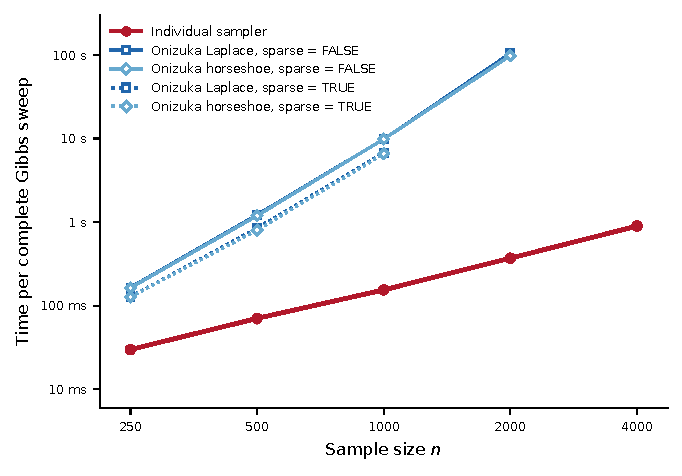
\includegraphics[width=0.78\textwidth]{figures/cost_scaling.pdf}
\caption{Median time per complete Gibbs sweep against sample size on log--log axes, with vertical bars spanning the range across repetitions (Table~\ref{tab:cost_scaling}). The supplied implementation of \citet{onizuka2024fast} grows as $n^{3.1}$ with \texttt{sparse = FALSE} and $n^{2.9}$ with \texttt{sparse = TRUE}; the individual sampler grows as $n^{1.22}$.}
\label{fig:cost_scaling}
\end{figure}

\paragraph{Results.} Table~\ref{tab:cost_scaling} and Figure~\ref{fig:cost_scaling} report the measurements. The ordering is not an artefact of one sample size, and the ratio widens with $n$ at the rate the operation counts predict. With its default settings the Laplace sampler of \citet{onizuka2024fast} takes 5.5 times as long per sweep as the individual sampler at $n = 250$, 17 times at $n = 500$, 63 times at $n = 1000$ and about 280 times at $n = 2000$, with the horseshoe sampler within a few percent of the Laplace sampler at every $n$; the two variants of the hierarchy differ in their scalar updates, which are not where the time goes. Over the measured range the supplied code grows as $n^{3.1}$ against $n^{1.22}$ for the individual sampler. Enabling the \texttt{sparse} option lowers the supplied code's time by 22--33\% at every $n$, which is the cost of the dense assembly products it removes, and leaves the growth at $n^{2.9}$: the inverse and the decomposition of the dense covariance remain, and they set the exponent.

The individual sampler's cost is where the analysis places it. The proximal calls account for 82--93\% of the measured time (Table~\ref{tab:prox_workload}). The number of inner ADMM iterations per sweep rises from 636 at $n = 250$ to 1297 at $n = 4000$; no call reached the $800$-iteration limit, the largest count for a single call being 740. The rise is not a failure of the solver but a consequence of the hierarchy: on this smooth signal the third differences of the trend are small, so the Gamma$(1 + m,\, 1 + S_D)$ full conditional places $\lambda$ near $m \approx n$, and the effective proximal penalty $\gamma\lambda$ grows with $n$. Together with the dense-$D$ term this accounts for the mild super-linearity of the individual sampler's growth: passing $D$ as a sparse matrix to the same code changes the time per sweep by at most 2\% for $n \le 1000$ and lowers it by 12\% at $n = 2000$ and $n = 4000$.

\begin{table}[!htbp]
\centering
\small
\caption{Proximal workload of the individual sampler across sample sizes (dense $D$; medians over repetitions unless stated). The inner-iteration count per sweep sums the three proximal calls; the per-call mean and maximum are over all calls in the measured windows; the proximal share is the fraction of measured time spent inside \texttt{glmgen::trendfilter}; acceptance is the P-MALA acceptance rate in the measured window, with the range across repetitions; $\bar\lambda$ is the mean of the sampled penalty over the window and $\delta$ the frozen step size. No call reached the $800$-iteration limit at any $n$.}
\label{tab:prox_workload}
\begin{tabular}{rrrrrrrr}
\toprule
$n$ & Inner & Mean & Max & Proximal & Acceptance & $\bar\lambda$ & $\delta$ \\
 & per sweep & per call & per call & share & & & \\
\midrule
250 & 636 & 212 & 386 & 91\% & 0.44 (0.38--0.64) & 245 & 0.045 \\
500 & 829 & 276 & 415 & 93\% & 0.52 (0.44--0.58) & 494 & 0.037 \\
1000 & 952 & 317 & 472 & 92\% & 0.42 (0.24--0.64) & 995 & 0.035 \\
2000 & 1097 & 366 & 611 & 88\% & 0.36 (0.26--0.38) & 1990 & 0.031 \\
4000 & 1297 & 432 & 740 & 82\% & 0.46 (0.32--0.50) & 4001 & 0.018 \\
\bottomrule
\end{tabular}
\end{table}

\paragraph{What these timings do and do not establish.} Time per sweep is not time per effective draw. The individual sampler's $\theta$ update is a Metropolis-within-Gibbs step with acceptance rate near $0.45$, whereas \citet{onizuka2024fast} draw $\theta$ from an exact full conditional, so equal sweep counts need not carry equal information, and a comparison in effective sample size per second requires mixing diagnostics that are not reported here. The gap measured above is, moreover, a property of the supplied implementation rather than of the locally adaptive hierarchy: a banded Gaussian draw is available for that hierarchy in $O(n)$ work, and a plain R re-implementation of the $\theta$ block along those lines, timed in the same session but not tabulated here because it is not the competitor's code, ran at 31~ms per sweep for the Laplace variant at $n = 1000$ and 122~ms at $n = 4000$, against 155 and 897~ms for the individual sampler. The per-sweep advantage of the proximal sampler is therefore over the implementation that was benchmarked in Section~\ref{sec:simulations}, and the fair asymptotic statement is that both schemes admit linear work per sweep at fixed $k$, the individual sampler with a constant governed by $J$ and the hierarchy with a constant governed by its $O(n)$ latent-variable and local-scale draws. The timings measure the computational work of the kernels as implemented, including the form of the P-MALA proposal used in Section~\ref{sec:simulations}; they are not a statement about the cost of a kernel whose invariant distribution has been separately verified. The two hierarchies differ in boundary treatment and in their scale and shrinkage priors, so the comparison is between two complete procedures and not between two implementations of one algorithm. Finally, the measurements are for one data set, one quantile level and one difference order; the inner iteration count, and with it the individual sampler's cost, will differ at other quantile levels and for other signals.
